\subsection{Intervalle}
\begin{defi}{Intervalle borné}{}
	Soit $a, b\in\R$ des réels avec $a\le b$. Soit $I$ l'ensemble des nombres réels compris entre $a$ et $b$. Les extrémités peuvent appartenir à $I$ ou pas. On dit que $I$ est un \bf{intervalle borné}.
\end{defi}

\begin{notation}{}{}
	On note un intervalle avec les extrémités entre crochets. Le crochet est tourné vers l'interieur lorsque l'extrémité appartient à l'intervalle.
\end{notation}

\begin{ex}{}{}
	Il y a donc quatre types d'intervalles bornés:
		\begin{itemize}
			\item L'ensemble des nombres réels $x\in\R$ tels que $a\le x\le b$. On le note $I = \{x\in\R, a\le x\le b\} = \ff{a}{b}$. Les deux extrémités appartiennent à $I$.
			\item  L'ensemble des nombres réels $x\in\R$ tels que $a<x\le b$. On le note $I = \{x\in\R, a< x\le b\}= \of{a}{b}$. $b$ appartient à $I$ mais pas $a$.
			\item L'ensemble $I = \{x\in\R, a\le x< b\}= \fo{a}{b}$.
			\item L'ensemble $I = \{x\in\R, a< x< b\}= \oo{a}{b}$.
		\end{itemize}
\end{ex}

\begin{ex}{}{}
	$I = \ff{0}{5}$ est l'ensemble des nombres entre 0 et 5. Il y a par exemple $0, 3/5, 4.1235456$ dedans.


	$J =\fo{0}{\pi}$ est l'ensemble des nombres positifs strictement plus petits que $\pi$. 
\end{ex}


\begin{defi}{Intervalle non borné}{}
	Soit $a\in\R$ un réel. Soit $I$ l'ensemble des nombres réels plus grand que $a$. L'extrémité $a$ peut appartenir à $I$ ou pas. De même, on définit l'ensemble $J$ des nombres réels plus petis que $a$.
	
	On dit que $I$ et $J$ sont des \bf{intervalles non bornés}.
\end{defi}

\begin{notation}{}{}
	Pour un intervalle non borné, on remplace une extrémité par $+\inf$ ou $-\inf$. Le crochet est toujours ouvert de ce côté, car l'infini n'est pas un nombre réel.
\end{notation}

\begin{exs}{}{}
	$I = \oo{0}{+\inf}$ est l'ensemble des nombres positifs.

	$I = \oo{-\inf}{5}$ est l'ensemble des nombres strictement plus petits que $5$.
\end{exs}


\begin{prop}{}{}
	Un intervalle borné correspond à un segment de la droite réelle.
	
	Un intervalle non borné correspond à une demi-droite ou a la droite réelle entière.
\end{prop}

\begin{ex}{}{}
\begin{center}
		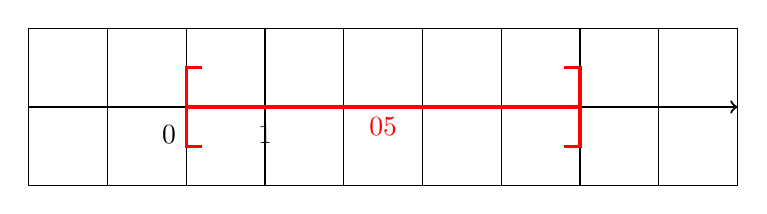
\begin{tikzpicture}
    	\draw (-2,-1) grid (7,1);
    	\draw[->, thick] (-2,0) -- (7,0);
    	\draw[thick] (0, 0.1) -- (0, -0.1) node [below left] {0};
    	\draw[thick] (1, 0.1) -- (1, -0.1) node [below] {1};
    	\draw[red, very thick] (0, 0) --  node [below] {$\ff{0}{5}$} (5, -0);
    	\draw[red, very thick] (0.2, 0.5) --  (0, 0.5) -- (0, -0.5) -- (0.2, -0.5);
    	\draw[red, very thick] (4.8, 0.5) --  (5, 0.5) -- (5, -0.5) -- (4.8, -0.5);
		\end{tikzpicture}
        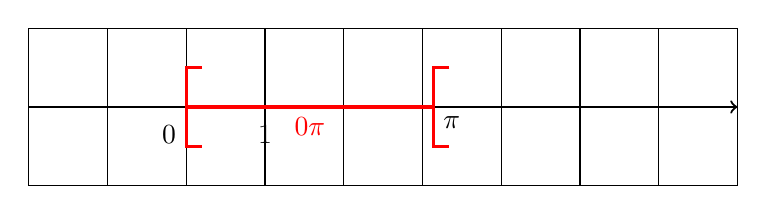
\begin{tikzpicture}
    	\draw (-2,-1) grid (7,1);
    	\draw[->, thick] (-2,0) -- (7,0);
        \node [below right] at (3.14, 0) {$\pi$};
    	\draw[thick] (0, 0.1) -- (0, -0.1) node [below left] {0};
    	\draw[thick] (1, 0.1) -- (1, -0.1) node [below] {1};
    	\draw[red, very thick] (0, 0) --  node [below] {$\fo{0}{\pi}$} (3.14, -0);
    	\draw[red, very thick] (0.2, 0.5) --  (0, 0.5) -- (0, -0.5) -- (0.2, -0.5);
    	\draw[red, very thick] (3.34, 0.5) --  (3.14, 0.5) -- (3.14, -0.5) -- (3.34, -0.5);
		\end{tikzpicture}
        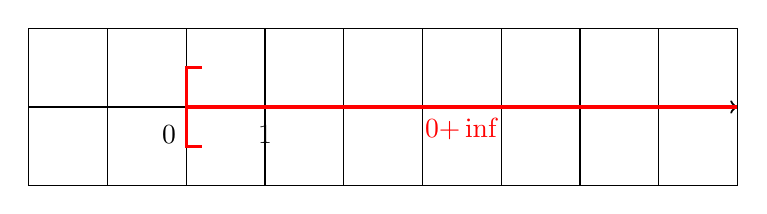
\begin{tikzpicture}
    	\draw (-2,-1) grid (7,1);
    	\draw[->, thick] (-2,0) -- (7,0);
    	\draw[thick] (0, 0.1) -- (0, -0.1) node [below left] {0};
    	\draw[thick] (1, 0.1) -- (1, -0.1) node [below] {1};
    	\draw[red, very thick] (0.2, 0.5) --  (0, 0.5) -- (0, -0.5) -- (0.2, -0.5);
    	\draw[red, very thick] (0, 0) --  node [below] {$\oo{0}{+\inf}$} (7, -0);
		\end{tikzpicture}
	\end{center}
\end{ex}

\begin{rem}{}{}
	Un intervalle est donc une partie "sans trous" de l'ensemble des nombres réels $\mathbb{R}$.
\end{rem}

\subsection{Distance entre deux nombres réels, notation $|a|$}

\begin{defi}{}{}
Soit $a$ un nombre réel.

 On appelle valeur absolue de $a$, notée $|a|$, la distance entre $a$ et $0$
\end{defi}

\smallskip
\begin{ex}{}{}
Essayons de déterminer $|-12|$.\medskip 

 On sait d'après la définition précédente que $|-12|$ est la \\distance entre $0$ et $-12$. On représente la droite des réels, \\puis (en rouge) la distance entre $0$ et $-12$:

\vspace{-15mm}
\begin{flushright}
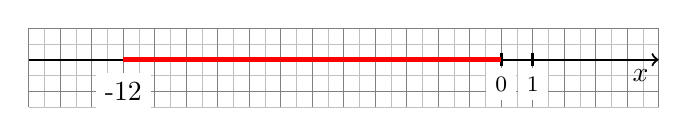
\begin{tikzpicture}[scale=0.4]
\def\xY{-15};
\def\yY{-1.5};
\def\xZ{5};
\def\yZ{1};
\coordinate (Y) at (\xY,\yY);
\coordinate (Z) at (\xZ,\yZ);
\draw[step=0.5cm, lightgray, very thin] (Y) grid (Z);
\draw[step=1cm, gray,thin] (Y) grid (Z);
\draw[ ->,thick] (\xY, 0) -- (\xZ, 0) node[below left]{$x$};
\foreach \x in {0,1}	\draw[very thick](\x,0.2cm)--(\x,-0.2cm) node[below,fill=white]{\footnotesize \x};
\def\xbornea{-12};
\def\orientationa{1};
\draw(\xbornea,-1)node[fill=white]{\xbornea};
\def\xborneb{0};
\def\orientationb{1};
\draw[line width=2pt,red](\xbornea,0)--(\xborneb,0);
\end{tikzpicture}
\end{flushright}

 On remarque que, bien que $-12$ soit négatif, $|-12|$ est positif et est égale à $12$. En effet, $|-12|$ est une distance donc toujours positive.
\end{ex}

\begin{rem}{}{}
Quelle que soit l'expression $a$, $a^2$ est toujours positive, donc $\sqrt{a^2}$ existe. Par exemple $\sqrt{3^2} = \sqrt{9} = 3$.

 On peut donc en déduire une autre manière de définir la valeur absolue: \quad $|a| = \sqrt{a^2}$
\end{rem}

\bigskip
 Plus généralement, avec la notation valeur absolue, il est possible de définir la distance entre deux nombres réels:

\begin{prop}{}{}
Soient $a$ et $b$ deux nombres réels. $|a-b|$ ou $|b-a|$ est la distance entre $a$ et $b$ 
\end{prop}

\smallskip
\begin{ex}{}{}
Essayons de déterminer $|2-11|$.\medskip 

 On sait d'après la définition précédente que $|2-11|$ est la \\distance entre $2$ et $11$. On représente la droite des réel, \\puis (en rouge) la distance entre $2$ et $11$:
\\
\vspace{-19mm}
\begin{flushright}
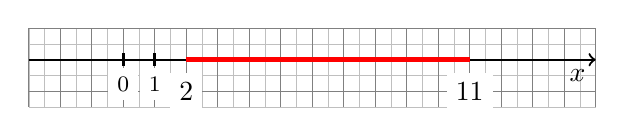
\begin{tikzpicture}[scale=0.4]
\def\xY{-3};
\def\yY{-1.5};
\def\xZ{15};
\def\yZ{1};
\coordinate (Y) at (\xY,\yY);
\coordinate (Z) at (\xZ,\yZ);
\draw[step=0.5cm, lightgray, very thin] (Y) grid (Z);
\draw[step=1cm, gray,thin] (Y) grid (Z);
\draw[ ->,thick] (\xY, 0) -- (\xZ, 0) node[below left]{$x$};
\foreach \x in {0,1}	\draw[very thick](\x,0.2cm)--(\x,-0.2cm) node[below,fill=white]{\footnotesize \x};
\def\xbornea{2};
\def\orientationa{1};
\draw(\xbornea,-1)node[fill=white]{\xbornea};
\def\xborneb{11};
\def\orientationb{1};
\draw(\xborneb,-1)node[fill=white]{\xborneb};
\draw[line width=2pt,red](\xbornea,0)--(\xborneb,0);
\end{tikzpicture}
\end{flushright}

 La distance entre $2$ et $11$ vaut $9$. Donc $|2-11| = 9$
\end{ex}

\subsection{Notion d'intervalle centré}

\begin{defi}{}{}
Soient $a$ un nombre réel et $r$ un nombre réel positif. 

 L'intervalle \quad $[a-r;a+r]$ \quad est un intervalle centré en \quad $a$ \quad de longueur \quad $2r$.
\end{defi}

\smallskip
\begin{ex}{}{}
Essayons de représenter l'intervalle pour $a=7$ et $r=10$ soit l'intervalle $[7-10;7+10]$.\medskip 

 On représente la droite des réels, \\puis (en violet) la valeur $7$:

\vspace{-12mm}
\begin{flushright}
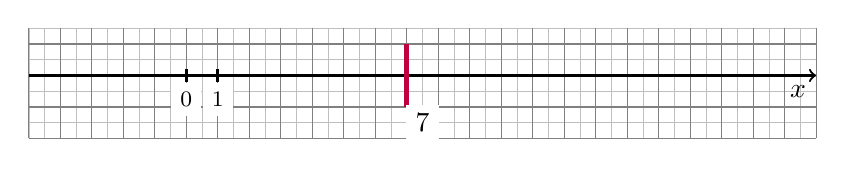
\begin{tikzpicture}[scale=0.4]
\def\xY{-5};
\def\yY{-2};
\def\xZ{20};
\def\yZ{1.5};
\coordinate (Y) at (\xY,\yY);
\coordinate (Z) at (\xZ,\yZ);
\draw[step=0.5cm, lightgray, very thin] (Y) grid (Z);
\draw[step=1cm, gray,thin] (Y) grid (Z);
\draw[ ->,thick] (\xY, 0) -- (\xZ, 0) node[below left]{$x$};
\foreach \x in {0,1}	\draw[very thick](\x,0.2cm)--(\x,-0.2cm) node[below,fill=white]{\footnotesize \x};
\def\xbornea{7};
\def\orientationa{1};
\draw[line width=1.7pt,purple] (\xbornea,1)--(\xbornea,-1);
\draw(\xbornea+0.5,-1.5)node[fill=white]{\xbornea};
\end{tikzpicture}
\end{flushright}


 On représente, en bleu, les valeurs comprises \\dans l'intervalle $[7-10;7]$ et, en rouge, les \\valeurs comprises dans l'intervalle $[7;7+10]$.

\vspace{-18mm}
\begin{flushright}
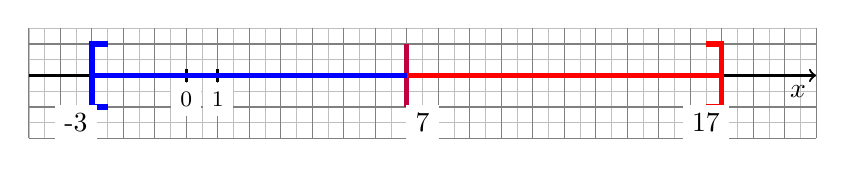
\begin{tikzpicture}[scale=0.4]
\def\xY{-5};
\def\yY{-2};
\def\xZ{20};
\def\yZ{1.5};
\coordinate (Y) at (\xY,\yY);
\coordinate (Z) at (\xZ,\yZ);\draw[step=0.5cm, lightgray, very thin] (Y) grid (Z);
\draw[step=1cm, gray,thin] (Y) grid (Z);
\draw[ ->,thick] (\xY, 0) -- (\xZ, 0) node[below left]{$x$};
\foreach \x in {0,1}	\draw[very thick](\x,0.2cm)--(\x,-0.2cm) node[below,fill=white]{\footnotesize \x};
\def\xbornea{7};
\def\orientationa{1};
\draw[line width=2pt,purple] (\xbornea,1)--(\xbornea,-1);
\draw(\xbornea+0.5,-1.5)node[fill=white]{\xbornea};
\def\xborneb{17};
\def\orientationb{1};
\draw[line width=2pt,red] ({\xborneb-0.5*\orientationb},1)--(\xborneb,1)--(\xborneb,-1)--({\xborneb-0.5*\orientationb},-1);
\draw(\xborneb-0.5,-1.5)node[fill=white]{\xborneb};
\draw[line width=2pt,red](\xbornea,0)--(\xborneb,0);
\def\xbornec{-3};
\def\orientationc{-1};
\draw[line width=2pt,blue] ({\xbornec-0.5*\orientationc},1)--(\xbornec,1)--(\xbornec,-1)--({\xbornec-0.5*\orientationc},-1);
\draw(\xbornec-0.5,-1.5)node[fill=white]{\xbornec};
\draw[line width=2pt,blue](\xbornea,0)--(\xbornec,0);
\end{tikzpicture}
\end{flushright}

\end{ex}

\medskip
Sur l'exemple précédent, on remarque que la distance entre la borne minimale, ici $-3$, et $7$ est la même que la distance entre la borne maximale de l'intervalle, ici $17$, et $7$.

 Cet intervalle est donc centré en $7$ et la distance entre le centre de l'intervalle et une borne est toujours inférieure ou égale à $10$. On peut donc définir ce genre d'intervalle grâce à la valeur absolue:

\begin{prop}{}{}
Soient $a$ un nombre réel et $r$ un nombre réel positif.

 L'intervalle \quad $[a-r;a+r]$ \quad peut être caractérisé par la condition:  \begin{center}
Pour tout $x \in \R$, $|x-a| \leqslant r$
\end{center}
\end{prop}
